\section{Propósito, alcance y diseño}
\label{sec:alcance}
\subsection{Pregunta y propósito analítico}

El proyecto busca describir cómo se distribuyen territorialmente las condiciones socioeconómicas observadas en 2018 y, en una fase posterior, estudiar su asociación con la contratación pública registrada en SECOP II durante 2026. La vulnerabilidad se entiende como una condición multidimensional relacionada con recursos, capacidades y exposición a restricciones; no es sinónimo automático de pobreza monetaria ni una característica individual que pueda inferirse directamente de un promedio municipal \citep{sen1999development,kaztman1999activos,pizarro2001vulnerabilidad}. El IPM municipal se conserva como referente externo para contraste posterior, no como insumo del PCA, para evitar validar una medida con componentes que reproducen su definición.

El estado del arte del proyecto aporta antecedentes de desigualdad regional y análisis territorial de pobreza y contratación. Se usan como contexto para formular la pregunta y justificar una lectura espacial, no como evidencia de que una combinación particular de variables sea válida para este IVS \citep{bonet2006desequilibrios,monsalvo2025ipm}.

\subsection{Diseño y unidad de inferencia}

La fase censal es transversal, descriptiva y ecológica: cada fila representa un código territorial y las observaciones describen agregados del CNPV 2018. Las asociaciones obtenidas no permiten atribuir características a hogares o personas específicas ni sostener causalidad. El IVS pretende resumir diferencias territoriales, no medir directamente la vulnerabilidad de cada residente.

El corte 2018 es la referencia socioeconómica del índice. SECOP II se mantendrá como bloque de análisis posterior y, por decisión del equipo, se priorizarán contratos de 2026. La diferencia temporal entre 2018 y 2026 exige interpretar el resultado como asociación entre una condición censal de referencia y una distribución contractual posterior, no como comparación contemporánea ni efecto causal.

\subsection{Fundamento estadístico de un índice compuesto}

Un indicador compuesto requiere definir constructo, cobertura, selección, normalización, agregación y sensibilidad; una técnica de ponderación no reemplaza las decisiones conceptuales \citep{booysen2002overview,oecd2008composite}. El PCA es una transformación lineal que produce combinaciones ortogonales ordenadas por varianza explicada. No identifica por sí mismo dimensiones de vulnerabilidad ni asigna pesos normativos justos. Por ello, se propone como procedimiento exploratorio condicionado a la coherencia de las variables, su estructura de correlación, su estabilidad y la interpretación de las cargas \citep{jolliffe2002principal,abdi2010principal}.

La escala 0--1 facilita leer cada proporción y orientar su significado. La matriz z pone las variables en varianza unitaria para que las diferencias de unidades no determinen la solución. La estandarización no homogeneiza la calidad del dato, no convierte una proxy en constructo validado y no significa que el efecto sustantivo de todas las variables deba ser igual.

\subsection{Trazabilidad de estados de evidencia}

En el informe se distinguen tres niveles: \textbf{verificado en archivo} (se reproduce desde una fuente o salida), \textbf{decisión acordada} (regla analítica adoptada por el equipo) e \textbf{interpretación o hipótesis} (lectura conceptual que deberá contrastarse). Una comprobación aritmética no se presenta como validación teórica; una decisión de ponderación tampoco se atribuye al DANE.


\section{Fuentes, extracción y organización de datos}
\label{sec:fuentes_extraccion}
\subsection{Fuentes primarias y su función}

La fuente socioeconómica principal es el CNPV 2018 publicado por el DANE, cuya cobertura y conceptos se rigen por la metodología censal oficial \citep{dane2021cnpv}. Se trabajó con dos libros consolidados: \path{datos/CUADROS_MUNICIPALES_UNIDOS.xlsx}, que reúne cuadros de hogares, personas y viviendas, y \path{datos/IPM_2018_organizado_region.xlsx}, que contiene el IPM municipal, desagregaciones, diccionarios y controles. \path{datos/DIVIPOLA-_Códigos_municipios_20260917.csv} se usa para contrastar códigos y nombres con la nomenclatura territorial de 2026, no para reemplazar silenciosamente la geografía censal de 2018. La fecha y estructura de los insumos quedan en las auditorías del repositorio.

Los cuadros seleccionados para la fase de indicadores son 1HM y 2HM (hogares), 5PM (actividad de personas de 10 años y más), 6V\_MPIO (material de paredes), 8V\_MPIO (servicios), 10V\_MPIO (estrato), y 17PM (nivel educativo). 1PM y 1V\_MPIO aportan denominadores y contexto. 6PM se excluyó por decisión del equipo: presenta variables coincidentes con 5PM, desagregadas por rangos de edad, y no se sumará como una dimensión adicional.

\subsection{Extracción y tipado}

Las tablas intermedias se producen con \path{R/01_verificar_consolidados.R}. Los libros se leen como texto para preservar ceros iniciales de códigos y se convierten las medidas a valores numéricos explícitamente. Las fórmulas de las columnas designadas en VIVIENDAS se verifican contra sus valores almacenados y sus componentes. Las filas \enquote{Total Nacional} se mantienen como controles, no como territorios. Cada bloque horizontal de VIVIENDAS y CONTEXTO se extrae con su propia llave y universo de filas.

La llave analítica es \texttt{codigo\_municipio} como cadena de cinco caracteres. La construcción y verificación se basan en códigos, no en nombres. Se conservan por separado código y nombre originales y se documentan las transformaciones. Las salidas tidy se organizan en \path{datos/intermedio/}; las salidas de inventario, cobertura y consistencia, en \path{resultados/verificacion_consolidados/}.

\subsection{Diccionario de variables y flujo de decisión}

El archivo \path{datos/Indices de bases y filas.xlsx} sirvió para localizar cuadros, hojas y rangos de filas/columnas en los libros fuente. A partir de ese mapa se actualizó \path{docs/diccionario/decisiones_variables_IVS_CNPV2018.csv}, que documenta para cada cuadro si se incluye, se conserva como contexto, se usa para validación o se descarta, junto con motivo y descripción. El diccionario es la capa de trazabilidad entre tabla censal, concepto, indicador y decisión del equipo; no es una autorización estadística automática para combinar variables.

La selección prioriza disponibilidad municipal, denominadores interpretables, comparabilidad y distancia conceptual frente al IPM. Los componentes del IPM no entran a la matriz candidata. Los cuadros del CNPV que coinciden directamente con privaciones del IPM pueden conservarse para descripción o contraste, pero no se duplican automáticamente dentro del IVS.

\begin{figure}[htbp]
\centering
\fbox{\begin{minipage}{0.94\textwidth}\centering
\textbf{Flujo reproducible de preparación}\par\vspace{0.4em}
Fuentes DANE / IPM / DIVIPOLA\par $\downarrow$\par
Inventario de hojas, extracción textual y llave territorial\par $\downarrow$\par
Tablas tidy + verificaciones de cobertura y consistencia\par $\downarrow$\par
Diccionario de decisiones + fórmulas explícitas\par $\downarrow$\par
Indicadores 0--1 + sensibilidades + matriz z\par $\downarrow$\par
\textbf{Submatriz de ocho candidatos y universo municipal por definir}\par $\downarrow$\par
PCA exploratorio (pendiente; no equivale a IVS validado)
\end{minipage}}
\caption{Etapas realizadas y transición pendiente hacia el PCA.}
\label{fig:flujo_metodologico}
\end{figure}


\section{Universo territorial, llaves y armonización}
\label{sec:universo_llaves}
\subsection{Universo censal y códigos de enlace}

El universo CNPV/IPM usado en la corrida del 15 de octubre comprende 1.122 códigos territoriales únicos. Este conteo no debe llamarse sin matices \enquote{1.122 municipios}: incluye áreas no municipalizadas y una unidad insular. La unión de ese universo con DIVIPOLA 2026 contiene un código adicional, 27493, exclusivo de la nomenclatura actual; el CNPV/IPM conserva 94663, que no aparece en DIVIPOLA 2026. La auditoría registra la fila completa de cada fuente y mantiene ambas situaciones visibles.

\begin{table}[htbp]
\centering\small
\caption{Casos territoriales que requieren armonización temporal}
\label{tab:casos_territoriales}
\begin{adjustbox}{max width=\textwidth}
\begin{tabular}{@{}p{0.12\textwidth}p{0.20\textwidth}p{0.25\textwidth}p{0.33\textwidth}@{}}
\toprule
\textbf{Código} & \textbf{Evidencia censal / DIVIPOLA} & \textbf{Decisión del equipo} & \textbf{Tratamiento y límite} \\
\midrule
27493 & Está en DIVIPOLA 2026; no en CNPV/IPM 2018. DANE incorporó Nuevo Belén de Bajirá a ELIC desde enero de 2024; no se sostiene aquí la fecha de creación 2019 previamente aportada \citep{dane2024elic}. & Enlace hacia 27615 (Riosucio) propuesto por el equipo, pendiente de verificación territorial. & No se inventa una observación censal 2018 ni se divide el dato de 27615. Deben verificarse acto de creación, límites y territorio antecedente antes de fijar el crosswalk. \\
94663 & Está en CNPV/IPM 2018; no en DIVIPOLA 2026. Corresponde a Mapiripana según el registro censal y la información aportada. & Enlace hacia 94343 (Barrancominas) para la geografía posterior. & Ambos códigos originales se preservan en la base de 2018. Para comparar con 2026 se requiere llevar las observaciones a geografía común; no se asignan contratos a unidades históricas que ya no tienen código vigente. \\
\bottomrule
\end{tabular}
\end{adjustbox}
\end{table}

La regla estadística general es conservar intacta la unidad observada por el CNPV 2018 y crear una capa separada de armonización para el enlace con SECOP II. Si una unidad de 2026 se divide respecto de 2018, los contratos de sus sucesores deben agregarse a la unidad histórica; si varias unidades de 2018 convergen en una de 2026, los conteos censales pertinentes deben agregarse primero y las tasas deben recalcularse como razón de sumas de numeradores y denominadores. No se deben promediar índices municipales ni repartir contratos proporcionalmente sin una regla y fuente justificadas. Este procedimiento es una especificación futura; no se ha ejecutado todavía.

La decisión del equipo es analizar las áreas no municipalizadas por separado del IVS municipal principal. La actualización descrita en la \cref{sec:actualizacion_descriptiva} verifica veinte ANM en la capa histórica DANE 2018, incluidas Barrancominas y Mapiripana. El DANE documenta que ambas integran Barrancominas bajo la Ordenanza 248 de 2019 \citep{dane2018divipola,dane_nbi_barrancominas}. Se generan descriptivos separados y una base municipal e insular de ocho indicadores; la inclusión de San Andrés en el futuro PCA aún debe declararse. DIVIPOLA 2026 no sustituye la clasificación histórica.

\subsection{Llaves, cobertura y áreas inexistentes}

El código se normaliza a cinco caracteres; el código departamental corresponde a sus dos primeros caracteres. Los nombres se conservan como atributos descriptivos, nunca como llave de unión. Las discrepancias ortográficas entre IPM y DIVIPOLA no cambian la correspondencia cuando el código coincide.

La auditoría CNPV/IPM registra 1.102 unidades con área Cabecera, 930 con Centro poblado, y los 1.122 códigos con Total y Rural disperso. Las ausencias de área se tratan como inexistencia estructural del dominio, no como no respuesta ni como ceros observados. En particular, los 20 códigos sin Cabecera coinciden con los 20 valores \enquote{--} de Cabeceras en el IPM. La clasificación de ANM, isla y municipios debe mantenerse ligada al registro temporal de referencia para no confundir cobertura censal con estado administrativo actual.

\subsection{Alcance de la cobertura SECOP II}

El criterio del equipo es exigir cobertura del 100\% del universo analítico acordado para el enlace principal con SECOP II y presentar sensibilidad si la armonización territorial reduce la cobertura. El denominador de ese porcentaje se definirá después de separar las ANM, resolver el universo municipal de referencia y fijar el crosswalk. Así se evita declarar cobertura completa contando simultáneamente unidades que representan territorios superpuestos o cambiados.


\section{Diccionarios y decisiones sobre variables}
\label{sec:seleccion_variables}
\subsection{Cuadros incluidos, contextuales y descartados}

El diccionario actualizado codifica el papel analítico de los cuadros. 1HM, 2HM, 5PM, 6V\_MPIO, 8V\_MPIO y 10V\_MPIO generan candidatas; 17PM queda como medida educativa descriptiva y candidata reservada para sensibilidad. 1PM se usa como contexto y fuente de denominadores, y 1V\_MPIO únicamente como contexto. 6PM se excluye: sus variables son equivalentes a 5PM pero organizadas por grupos de edad, por lo que incluirlo como otra medida duplicaría la dimensión observada. El IPM se guarda para validación externa; sus 15 privaciones no se suman al PCA.

En 6V\_MPIO se mantiene el conjunto de seis categorías acordado por el equipo: guadua; tapia pisada/bahareque/adobe; madera burda/tabla/tablón; caña, esterilla y otros vegetales; materiales de desecho; y sin paredes. La elección agrupa materiales que requieren interpretación conjunta y no afirma que tengan idéntica severidad. El solapamiento directo con la privación IPM de paredes se evaluará externamente.

En 8V\_MPIO se analizan por separado energía, gas e internet. Acueducto y alcantarillado quedan fuera de la matriz principal por cercanía conceptual con privaciones IPM, pero se conservan como variables descriptivas. Las categorías \enquote{Sin información} permanecen registradas; no se confunden con viviendas que carecen del servicio.

La decisión confirmada el 18 de octubre asigna recolección de basuras únicamente a sensibilidad exploratoria. La matriz histórica de siete variables la incluía; las ocho actuales la retiran e incorporan 2HM y 6V, además de revisar fórmulas de actividad y estrato. Por ello, los diagnósticos históricos no son aplicables automáticamente a la especificación actual. Este acuerdo posterior se registra en la actualización del informe y en su nota de decisiones; el CSV histórico se conserva para trazabilidad.

\subsection{Dirección conceptual}

Las candidatas se orientan para que valores altos indiquen mayor condición potencial de vulnerabilidad según la operacionalización acordada. Esta orientación es una convención explícita del estudio, no una constatación causal. En particular, tener menores o personas mayores en el hogar representa una posible carga de cuidado, pero no demuestra dependencia económica ni funcional. El estrato es una clasificación administrativa del inmueble residencial asociada con servicios públicos; la inclusión de \enquote{no tiene estrato} como vulnerabilidad es una decisión del proyecto, no una consecuencia automática de la Ley 142 ni una medición directa del ingreso \citep{dane_estratificacion}.

En 5PM, la variable censal clasifica la actividad realizada la semana anterior por población de 10 años y más. El agregado propuesto mezcla trabajo no remunerado, búsqueda de empleo e incapacidad permanente con mayor ponderación de esta última. Por tanto, es una puntuación experimental municipal y no debe nombrarse tasa de desempleo, dependencia económica del hogar ni \enquote{última actividad laboral del hogar}. El cuadro no contiene el vínculo persona-hogar necesario para esa última interpretación \citep{dane_5pm}.

17PM mide nivel educativo alcanzado en población de cinco años y más. Sus categorías por municipio, área y sexo no están desagregadas por edad en el cuadro utilizado. La proporción agregada puede variar por la composición etaria además de las oportunidades educativas; por ello no se interpreta como educación ajustada por edad ni como asistencia escolar. La candidata agregada \texttt{sin\_media\_completa\_17PM} queda fuera del primer PCA, pendiente de análisis exploratorio de sensibilidad.

\subsection{Diccionario operativo de variables y siglas}
\label{subsec:diccionario_operativo}

Este diccionario traduce los códigos de los cuadros del CNPV 2018 y las variables empleadas en el análisis a definiciones legibles. Los códigos \textbf{1HM, 2HM, 5PM, 6V\_MPIO, 8V\_MPIO, 10V\_MPIO, 17PM, 1PM y 1V\_MPIO} son identificadores de cuadros o decisiones, no nombres de indicadores oficiales. Las definiciones censales y sus universos se toman de la documentación del DANE; la dirección de vulnerabilidad y las agrupaciones descritas como decisiones del equipo son operacionalizaciones del estudio \citep{dane2021cnpv,dane2020ipmcensal,dane_5pm}.

La expresión \textbf{Total} en las tablas siguientes identifica el dominio municipal del cuadro, frente a Cabecera, Centro poblado y Rural disperso. No significa necesariamente que dos cuadros midan el mismo universo: hogares, viviendas, personas de 10+ y personas de 5+ tienen denominadores diferentes. Por ello, los numeradores y denominadores de cada indicador se interpretan dentro de su propio cuadro.

\begin{singlespace}
\small
\begin{longtable}{@{}p{0.13\textwidth}p{0.22\textwidth}p{0.36\textwidth}p{0.21\textwidth}@{}}
\caption{Diccionario de cuadros, variables y uso analítico}\label{tab:diccionario_operativo}\\
\toprule
\textbf{Código / variable} & \textbf{Qué significa} & \textbf{Definición operativa y universo} & \textbf{Uso e interpretación en el proyecto}\\
\midrule
\endfirsthead
\toprule
\textbf{Código / variable} & \textbf{Qué significa} & \textbf{Definición operativa y universo} & \textbf{Uso e interpretación en el proyecto}\\
\midrule
\endhead
\midrule
\multicolumn{4}{r}{Continúa en la página siguiente}\\
\endfoot
\bottomrule
\endlastfoot
1HM & Hogares con menores de 15 años & Número de hogares que reportan al menos una persona menor de 15, dividido por el total de hogares del mismo dominio. El cuadro también registra número de menores de 15. & Candidata principal. Aproxima presencia de posibles necesidades de cuidado; no mide dependencia económica, cuidado efectivamente prestado ni número de menores por hogar.\\
2HM & Hogares con personas de 60 años o más & Hogares con al menos una persona de 60+ dividido por el total de hogares. El cuadro registra asimismo personas de 60+. & Candidata principal. Proxy de carga potencial de cuidado. La edad por sí sola no establece discapacidad, dependencia funcional ni necesidad de apoyo.\\
Hogares totales (1HM/2HM) & Denominador de hogares & Total censal de hogares particulares del área Total del cuadro de hogares; no es el total de viviendas ni la población. & Denominador específico de 1HM y 2HM.\\
5PM & Actividad realizada la semana anterior & Distribución de actividades declaradas para población de 10 años o más: no informa; trabajó al menos una hora; trabajó o ayudó sin remuneración; tenía empleo pero no trabajó; buscó trabajo; vivió de jubilación/pensión/renta; estudió; realizó oficios del hogar; incapacidad permanente; otra situación. & El agregado municipal ponderado es experimental. No equivale a tasa oficial de desempleo, actividad laboral actual ni dependencia económica del hogar.\\
No remunerado (5PM) & Trabajo o ayuda sin remuneración & Personas de 10+ que trabajaron o ayudaron en un negocio por lo menos una hora sin recibir pago, según la categoría censal. & Componente del numerador de 5PM con peso 1. No es por sí solo una medida de vulnerabilidad.\\
Búsqueda (5PM) & Buscó trabajo & Personas de 10+ que declararon buscar trabajo la semana anterior. & Componente del numerador de 5PM con peso 1; no constituye por sí solo el desempleo oficial.\\
Incapacidad permanente (5PM) & Incapacitado(a) permanentemente para trabajar & Categoría de actividad declarada por población de 10+. & Componente de 5PM con peso 2 por acuerdo normativo del equipo; ese peso no es estimado ni validado como óptimo.\\
No informa (5PM) & Sin clasificación de actividad & Personas de 10+ ubicadas por el cuadro en la categoría No informa. & Se excluye del denominador válido de la fórmula aprobada y se conserva para documentar cobertura/no respuesta.\\
6V\_MPIO & Material predominante de paredes exteriores & Conteos de viviendas por material predominante, para los tipos de vivienda del cuadro y dominios geográficos. & Candidata principal agregada. El nombre operativo \path{paredes_precarias_6V} es una etiqueta del proyecto, no categoría oficial del DANE ni juicio de que cada material sea inadecuado.\\
Seis materiales (6V) & Grupo de materiales acordado & Suma de: guadua; tapia pisada/bahareque/adobe; madera burda/tabla/tablón; caña/esterilla/otros vegetales; materiales de desecho; y sin paredes. & Numerador de la candidata agregada, dividido por el total de viviendas tipo Total de 6V. Se conservan desgloses para sensibilidad; no se presupone severidad idéntica.\\
Viviendas tipo Total (6V) & Universo de referencia de paredes & Total de viviendas clasificadas como tipo Total en el bloque 6V. & Denominador de la candidata de paredes. No confundir con viviendas ocupadas presentes del bloque 8V.\\
8V\_MPIO & Servicios públicos en viviendas ocupadas presentes & Conteos de viviendas ocupadas con personas presentes y categorías de respuesta por servicio. & Se consideran como candidatas separadas energía, gas e internet. Acueducto, alcantarillado y basuras no pertenecen a las ocho principales; basuras queda para sensibilidad exploratoria.\\
Sin energía (8V) & Viviendas sin servicio de energía eléctrica & Conteo de respuesta No para energía, respecto del total de viviendas ocupadas con personas presentes. & Candidata principal de carencia declarada del servicio. No mide continuidad, calidad ni capacidad de pago.\\
Sin gas (8V) & Viviendas sin conexión a gas natural por red pública & Respuesta No en gas; el denominador aprobado es total de gas menos Sin información. & Candidata principal entre respuestas clasificables. No equivale a carecer de combustible o energía para cocinar; Sin información se conserva aparte.\\
Sin internet (8V) & Viviendas sin servicio de internet & Respuesta No en internet; denominador aprobado: total de internet menos Sin información. & Candidata principal entre respuestas clasificables. No mide calidad, uso ni habilidades digitales.\\
Acueducto / alcantarillado (8V) & Acceso declarado a esos servicios & Para cada servicio, el cuadro distingue total, Sí y No. & Variables conservadas en datos; excluidas de las ocho candidatas por decisión del equipo sobre proximidad conceptual con IPM.\\
Recolección de basuras (8V) & Servicio de recolección de residuos & Categorías Sí/No para viviendas ocupadas presentes. & Excluida de la matriz principal; sensibilidad exploratoria aprobada.\\
Sin información (8V) & Respuesta no clasificada para gas o internet & Categoría específica de no respuesta que el cuadro reporta en esos servicios. & No se recodifica como Sí o No. Se comparan escenarios con denominador válido y con el total; no respuesta no aleatoria no se descarta.\\
10V\_MPIO & Personas por condición de estrato de energía & Personas en hogares particulares clasificadas en estratos 1--6, sin servicio de energía, no tiene estrato o no sabe/no responde. El cuadro usa la grafía errónea \enquote{Perosnas} en un encabezado. & Candidata principal, con universo condicional explícito; clasificación socioeconómica del inmueble asociada a servicios, no medición directa del ingreso individual.\\
Estratos 1--2 (10V) & Categorías de estrato residencial bajo & Suma de personas en estrato 1 y estrato 2. & Parte del numerador acordado para 10V; el corte es una decisión operacional del proyecto.\\
No tiene estrato (10V) & Viviendas/personas sin clasificación de estrato & Categoría separada que el cuadro distingue de estratos 1--6 y de No sabe/No responde. & Se incluye en numerador y denominador de 10V por decisión del equipo. La inclusión no demuestra vulnerabilidad por sí misma.\\
Sin servicio / NS-NR (10V) & Sin energía; no sabe o no responde & Categorías distintas de estratos 1--6 y No tiene estrato. & Se excluyen del cociente principal, pero se conservan y se evalúa el efecto de incorporar categorías no clasificables en sensibilidad.\\
17PM & Nivel educativo alcanzado & Distribución por categorías educativas de la población de 5 años o más, por área y sexo. & Reservada para exploración descriptiva/sensibilidad; no mide asistencia escolar. La distribución agregada puede cambiar por composición etaria y las categorías son composicionales.\\
Sin media completa (17PM) & Agregado educativo candidato & Ninguno, preescolar, primaria completa/incompleta, secundaria completa/incompleta y media incompleta, sobre población de 5+. Normal incompleta se evalúa solo como sensibilidad; Normal completa queda fuera. & No entra al primer PCA. No está ajustada por edad y su asociación conceptual con privaciones educativas del IPM debe tratarse como cercanía, no validación independiente.\\
1PM & Población por edad y sexo & Conteos de población por grupos de edad y sexo, total y dominios del cuadro; incluye índices de masculinidad/feminidad. & Contexto y denominadores. No es indicador candidato de la matriz principal. Las categorías de edad sin fila en un bloque pueden representar cero casos/no registro estructural, no necesariamente NA.\\
1V\_MPIO & Tipo y condición de ocupación de vivienda & Conteo de viviendas por tipo y estado: ocupada con personas presentes, ocupada con personas ausentes, temporal para vacaciones y desocupada. & Solo contexto. No es candidata ni denominador intercambiable con 6V o 8V.\\
6PM & Actividad por grupos de edad & Desagregación de variables equivalentes a 5PM por grupos etarios. & Excluida por decisión del equipo para no duplicar el cuadro 5PM en la matriz principal.\\
IPM municipal & Índice de Pobreza Multidimensional & Medida oficial construida con privaciones definidas por DANE y regla de identificación del IPM; las variables publicadas incluyen resultado municipal y dominios. & Validador externo/convergente posterior, no componente de la matriz IVS. Comparte fuente censal con las candidatas, por tanto la validación no será completamente independiente.\\
Privaciones IPM & Indicadores de privación del hogar & Incluyen analfabetismo, bajo logro educativo, barreras a cuidado de primera infancia y salud, dependencia, hacinamiento, saneamiento, inasistencia y rezago escolar, materiales, agua, aseguramiento, trabajo infantil e informalidad. & Las quince se mantienen fuera del PCA. Se usan para contraste conceptual; el dominio compartido no implica igualdad de definición.\\
ANM & Área no municipalizada & Unidad territorial censal identificada como área no municipalizada en la geografía DIVIPOLA de 2018. & Se conserva y describe por separado; no se denomina municipio. La inclusión de San Andrés en descriptivos se informa aparte.\\
\bottomrule
\end{longtable}
\normalsize
\end{singlespace}

\paragraph{Abreviaturas de lectura.} \textbf{DE}: desviación estándar; \textbf{NR}: no respuesta; \textbf{NS-NR}: no sabe/no responde; \textbf{PCA}: análisis de componentes principales; \textbf{IPM}: Índice de Pobreza Multidimensional; \textbf{ANM}: área no municipalizada. Los nombres de variables de los CSV se mantienen en \texttt{snake\_case}; las etiquetas de este diccionario facilitan su interpretación sin alterar archivos ni fórmulas.

El inventario reproducible de variables fuente, columnas y nombres limpios está en los resultados de verificación de consolidados; este diccionario resume el significado analítico acordado. En caso de diferencia, prevalecen los encabezados y universos observados del CNPV, y la definición operacional citada en la tabla de fórmulas del informe.


\section{Indicadores candidatos y fórmulas}
\label{sec:indicadores}
\subsection{Reglas comunes}

Las fórmulas usan totales municipales del área \enquote{Total}; no se derivan tasas nuevas desde áreas parciales ni se suman denominadores de universos incompatibles. Los indicadores proporcionales se expresan en escala 0--1 y se orientan positivamente como mayor condición potencial de vulnerabilidad. La matriz z se obtiene estandarizando las columnas candidatas disponibles entre las unidades territoriales del archivo. Los denominadores cero no se convierten en valores artificiales; se conservan como indefinidos cuando aparecen.

\subsection{Especificación de candidatas}

\begin{singlespace}
\small
\begin{longtable}{@{}p{0.14\textwidth}p{0.32\textwidth}p{0.31\textwidth}p{0.12\textwidth}@{}}
\caption{Fórmulas de las nueve candidatas actualmente calculadas}\label{tab:formulas_candidatas}\\
\toprule
\textbf{Candidata} & \textbf{Numerador / denominador} & \textbf{Interpretación y cautela} & \textbf{Estado}\\
\midrule
\endfirsthead
\toprule
\textbf{Candidata} & \textbf{Numerador / denominador} & \textbf{Interpretación y cautela} & \textbf{Estado}\\
\midrule
\endhead
Hogares con menores de 15 & Hogares con menores de 15 / hogares totales (1HM). & Proxy de carga potencial de cuidado; no mide dependencia económica. & Primer PCA \\
Hogares con personas de 60+ & Hogares con adultos mayores / hogares totales (2HM). & Proxy de carga potencial de cuidado; edad no implica dependencia funcional. & Primer PCA \\
Paredes precarias (6V) & Viviendas con las seis categorías acordadas / viviendas tipo Total. & Indicador material agregado; no asume igual severidad de cada material. & Primer PCA \\
Sin energía (8V) & Viviendas ocupadas presentes sin energía / viviendas ocupadas presentes. & Carencia de servicio; considerar oferta e infraestructura local. & Primer PCA \\
Sin gas de red (8V) & Viviendas sin gas / (total de gas menos Sin información). & Proporción entre respuestas clasificables; NR conservada aparte. & Primer PCA \\
Sin internet (8V) & Viviendas sin internet / (total de internet menos Sin información). & Proporción entre respuestas clasificables; NR conservada aparte. & Primer PCA \\
Estratos 1--2 o sin estrato (10V) & Personas en estratos 1--2 más No tiene estrato / personas en estratos 1--6 más No tiene estrato. & Decisión operacional del equipo; Sin servicio y No sabe/No responde quedan fuera del cociente y se conservan por separado. & Primer PCA \\
Actividad ponderada 10+ (5PM) & (No remunerado + buscó trabajo + 2 $\times$ incapacidad permanente) / [2 $\times$ (población de 10+ menos No informa)]. & Puntuación experimental; ponderación 2:1 acordada por el equipo. No es tasa oficial de desempleo ni dependencia del hogar. & Primer PCA \\
Sin media completa (17PM) & Ninguno + preescolar + primaria completa/incompleta + secundaria completa/incompleta + media incompleta, dividido por población de 5+. & Mezcla edades; Normal incompleta solo en sensibilidad y Normal completa excluida del numerador. & Reservada \\
\bottomrule
\end{longtable}
\normalsize
\end{singlespace}

Las primeras ocho filas analíticas son las candidatas previstas para el primer PCA. La novena, educación, queda fuera hasta evaluar su sensibilidad. Las 15 proporciones educativas por categoría se almacenan descriptivamente; no se incorporan juntas en bruto porque comparten un denominador y suman uno. Esa restricción composicional induce dependencia matemática; un PCA convencional sobre todas las partes requiere transformación y tratamiento de ceros apropiados \citep{aitchison1983compositional}. El agregado de \enquote{sin media completa} reduce la dimensión, pero no elimina la confusión potencial por edad.

\subsection{Denominadores y alcance de 5PM}

El peso máximo por persona con respuesta válida en 5PM es dos, de modo que el denominador ponderado limita el puntaje a [0,1]. El peso 2 para incapacidad permanente es una ponderación normativa definida por los autores, no un parámetro estimado por el censo. La sensibilidad muestra que cambiarlo modifica de forma material la distribución municipal; por ello debe permanecer identificado como decisión experimental aun cuando se use en el primer análisis.

El 10V usa personas clasificadas en algún estrato o en \enquote{No tiene estrato}. Al excluir \enquote{Sin servicio de energía} y \enquote{No sabe/No responde}, el indicador describe la proporción de la población bajo la regla entre categorías clasificables, no entre todos los habitantes. Las dos categorías excluidas quedan como variables observables separadas y la sensibilidad del denominador total cuantifica cuánto cambiaría la medida si se las incorporara.


\section{Tratamiento de datos y sensibilidad}
\label{sec:tratamientos_sensibilidad}
\subsection{Ceros, no respuesta y ausencias estructurales}

Se distinguen valores cero observados, no respuesta explícita, celdas vacías, áreas inexistentes y denominadores sin población de referencia. La ausencia de una combinación área--tipo--grupo no se transforma automáticamente en cero. Las áreas geográficas inexistentes se excluyen del cálculo por área y se reportan como tales; un denominador cero produce cociente indefinido, no un cero imputado. Las categorías \enquote{Sin información}, \enquote{No informa} y \enquote{No sabe/No responde} se preservan y se analizan según la fórmula, sin ocultarlas dentro de categorías sustantivas.

En gas e internet la fórmula principal excluye NR del denominador y una alternativa divide por el total publicado. Esta comparación es una sensibilidad de fórmula; no reemplaza el análisis multivariado con y sin NR. Para estrato, \enquote{No tiene estrato} es una categoría distinta a no respuesta y entra en la candidata por decisión del equipo. No se aplicó imputación estadística en la matriz final de candidatos.

\subsection{Resultados históricos de sensibilidad, universo censal completo}

Las diferencias se calcularon a nivel de código territorial para 1.122 unidades. \enquote{Delta 2 pp} cuenta unidades cuya diferencia absoluta es al menos 0,02 en escala 0--1. $\rho_s$ es la correlación de rangos de Spearman entre la fórmula principal y la alternativa; no evalúa estabilidad de cargas o componentes PCA.

\begin{table}[htbp]
\centering\small
\caption{Sensibilidad de fórmulas y denominadores}\label{tab:sensibilidad}
\begin{adjustbox}{max width=\textwidth}
\begin{tabular}{@{}p{0.23\textwidth}p{0.34\textwidth}r r r r@{}}
\toprule
\textbf{Indicador} & \textbf{Comparación} & \textbf{$n$} & \textbf{$\rho_s$} & \textbf{Delta máx.} & \textbf{$\geq$2 pp}\\
\midrule
5PM ponderado & Excluir No informa vs. total & 1.122 & 0,999 & 0,0084 & 0 \\
5PM NR & Fórmula principal vs. cota que asigna máximo a NR & 1.122 & 0,813 & 0,1826 & 235 \\
5PM peso & Incapacidad 2:1 vs. 1:1 & 1.122 & 0,950 & 0,2143 & 702 \\
5PM peso & Incapacidad 2:1 vs. 3:1 & 1.122 & 0,976 & 0,0714 & 46 \\
Gas (8V) & Denominador válido vs. total & 1.122 & 0,994 & 0,1246 & 58 \\
Internet (8V) & Denominador válido vs. total & 1.122 & 0,954 & 0,1676 & 85 \\
Estrato (10V) & Categorías clasificables vs. total personas & 1.122 & 0,404 & 0,9880 & 711 \\
Educación (17PM) & Sin media completa vs. incluir Normal incompleta & 1.122 & 0,998 & 0,0479 & 12 \\
Educación (17PM) & Población 5+ vs. 5+ válida sin Sin información & 1.122 & 0,968 & 0,2141 & 105 \\
\bottomrule
\end{tabular}
\end{adjustbox}
\end{table}

La sensibilidad de 5PM indica que el peso de incapacidad sí altera la ordenación municipal y no queda resuelto solo por la alta correlación de rangos. La elección 2:1 se conserva porque fue aprobada por el equipo, con carácter explícitamente experimental. En 10V, el cambio extremo frente al denominador de todas las personas señala que la proporción depende mucho de la regla de elegibilidad; no se recomienda interpretar ambos denominadores como equivalentes. En 17PM, la variación por denominador y la composición etaria refuerzan la decisión de no llevarla al primer PCA.

\subsection{Alcance de la ampliación de sensibilidad}

Las cifras anteriores comparan valores de indicadores en el universo completo. La actualización de la \cref{sec:actualizacion_descriptiva} añade resultados para el ámbito municipal e insular y cambios en correlaciones de Pearson y Spearman. KMO/MSA, cargas, número de componentes y puntuaciones siguen pendientes. No se debe elegir una fórmula solo por su correlación de rangos con otra ni tratar la estabilidad de correlaciones como validación del futuro índice.


\section{Verificación y resultados reproducibles}
\label{sec:verificacion_resultados}
\subsection{Resultados de la corrida reproducible}

El producto \path{resultados/indicadores_finales_ivs_20261015/resumen_ejecucion.csv} registra 1.122 códigos, nueve columnas candidatas, quince proporciones educativas descriptivas, 1.122 filas completas, cero celdas NA, cero violaciones en los controles incluidos y \texttt{PCA\_ejecutado = FALSE}. 6PM no se incluye. Los nueve indicadores están dentro del rango previsto [0,1] y las quince partes de 17PM suman uno por código territorial.

\begin{table}[htbp]
\centering\small
\caption{Controles de consistencia de la matriz candidata}\label{tab:controles_matriz}
\begin{adjustbox}{max width=\textwidth}
\begin{tabular}{@{}p{0.54\textwidth}r r p{0.23\textwidth}@{}}
\toprule
\textbf{Control} & \textbf{$n$ evaluado} & \textbf{Violaciones} & \textbf{Tolerancia}\\
\midrule
Cobertura y unicidad de códigos entre fuentes & 1.122 & 0 & Exacta \\
Total 17PM = suma de categorías & 1.122 & 0 & 0,5 persona \\
Total 5PM = suma de categorías & 1.122 & 0 & 0,5 persona \\
Total 6V = suma de nueve materiales & 1.122 & 0 & 0,5 vivienda \\
Total energía 8V = Sí + No & 1.122 & 0 & 0,5 vivienda \\
Total gas e internet = Sí + No + Sin información & 2.244 & 0 & 0,5 vivienda \\
Total 10V = suma de categorías BU:CD & 1.122 & 0 & 0,5 persona \\
Indicadores candidatos en [0,1] & 10.098 celdas & 0 & [0,1] \\
Completitud de las nueve candidatas & 10.098 celdas & 0 NA & NA \\
\bottomrule
\end{tabular}
\end{adjustbox}
\end{table}

Estos controles verifican aritmética, rangos y cobertura de la matriz producida; no prueban que la operacionalización represente por completo la vulnerabilidad. Asimismo, la sensibilidad por denominador de estrato documenta una limitación conceptual importante: la población fuera de categorías clasificables no entra en el indicador principal.

\subsection{Qué se verificó en los consolidados}

La auditoría del consolidado verificó nombres de hojas, bloques, dimensión, formatos de llave, consistencia interna, coberturas por área y correspondencia entre hoja ancha y larga del IPM. El informe correspondiente es \path{docs/calidad/auditorias/VERIFICACION_CONSOLIDADOS.md}; sus archivos tabulares están en \path{resultados/verificacion_consolidados/}. El código se usa para unir y los nombres se emplean solo para describir. La ausencia de Cabecera en 20 unidades coincide con los 20 \enquote{--} del IPM, y la ausencia de Centro poblado en 192 unidades se conserva como falta de dominio geográfico, no de dato.

\subsection{Resultados que no se trasladan de versiones anteriores}

Los diagnósticos KMO, Bartlett, MSA, correlaciones y extremos que aparecen en la auditoría de la matriz previa se refieren a otra especificación. No se presentan aquí como resultados de las nueve candidatas actuales ni de la futura matriz de ocho variables. Los diagnósticos de adecuación deben recalcularse sobre el universo municipal depurado y la submatriz acordada antes de decidir si procede PCA.


\section{Decisiones consolidadas, descriptivos y sensibilidades al 18 de octubre}
\label{sec:actualizacion_descriptiva}
\subsection{Decisiones cerradas y alcance de esta actualización}

La actualización del 18 de octubre de 2026 conserva ocho candidatas: 1HM, 2HM, seis materiales agregados de 6V, energía, gas e internet de 8V, 10V y actividad ponderada 5PM. Basuras queda fuera de ese conjunto y se examina exclusivamente como sensibilidad exploratoria. Se mantiene 17PM reservada, 1PM y 1V como contexto, y 6PM excluida. Las quince privaciones del IPM permanecen fuera de la matriz. El equipo aprobó conservar las candidatas pese a su proximidad temática con el IPM, hacer explícita esa proximidad y comparar posteriormente soluciones que retiren las más cercanas. Esta corrida calcula descriptivos y sensibilidad de fórmulas y correlaciones; no ejecuta PCA, KMO, Bartlett ni construcción del IVS.

\subsection{Justificación específica y límites de las aproximaciones}

El marco de activos y oportunidades fundamenta una lectura multidimensional de restricciones y recursos \citep{kaztman1999activos,pizarro2001vulnerabilidad}. El antecedente colombiano ICVU incorpora cuidado, condiciones habitacionales y acceso a bienes; utiliza hogares y otro método, por lo que respalda la pertinencia de esos dominios, sin validar nuestras fórmulas municipales \citep{dnp2023icvu}. Para cada candidata se conserva la definición y el denominador de la \cref{tab:formulas_candidatas}, con las siguientes precisiones:

\begin{description}[leftmargin=1.27cm,style=nextline]
\item[1HM y 2HM: composición del hogar y cuidado potencial.] Son proporciones de hogares con presencia de los grupos de edad elegidos. Su dirección positiva es una hipótesis operacional del equipo. El antecedente sobre cuidado respalda explorar el dominio, pero la edad no determina necesidad de ayuda: no se observan horas de cuidado, autonomía, apoyos ni dependencia económica. Los hogares pueden pertenecer a ambas categorías; no son partes de una distribución exhaustiva \citep{dnp2023icvu,dane2021cnpv}.
\item[6V: composición material de las paredes.] Se mantiene la agregación de seis materiales aprobada. La calidad de vivienda es pertinente para estudiar condiciones de vida, pero el material aislado no informa estado constructivo, mantenimiento, riesgo local ni adecuación cultural. En particular, incluir guadua y tapia/bahareque/adobe no implica que toda construcción con esos materiales sea insegura. El nombre operativo \texttt{paredes\_precarias\_6V} designa la agrupación del proyecto, no una clasificación oficial de déficit. Se publican las seis proporciones para examinar sus contribuciones \citep{dane2021cnpv,dnp2023icvu}.
\item[Energía, gas e internet (8V): acceso diferenciado.] Las tres proporciones describen carencia declarada del servicio correspondiente entre viviendas ocupadas con personas presentes. La falta de gas por red puede relacionarse con oferta territorial y combustibles alternativos; no mide por sí sola falta de energía para cocinar. La ausencia de internet no informa calidad, uso ni habilidades digitales. Se conservan como aproximaciones diferenciadas y se examinan denominadores y correlaciones, sin atribuirles equivalencia sustantiva \citep{dane2021cnpv}.
\item[10V: clasificación socioeconómica asociada al inmueble.] El DANE fundamenta la estratificación en características del inmueble para servicios públicos. Esa finalidad respalda un uso contextual; no demuestra que todas las personas sin estrato sean vulnerables. El corte 1--2, la inclusión de \enquote{No tiene estrato} y la dirección positiva son decisiones del equipo. La proporción condiciona en estratos 1--6 más \enquote{No tiene estrato}; no mide prevalencia entre toda la población. Las categorías sin servicio de energía y no respuesta permanecen separadas. La Ley 142 no se utiliza como prueba de validez de este numerador \citep{dane_estratificacion}.
\item[5PM: puntuación experimental de actividad de población 10+.] Las categorías proceden de la actividad de la semana anterior. La suma ponderada representa una decisión operacional de relevancia relativa, sin identificar desempleo oficial ni dependencia de hogares. El peso 2:1 es normativo; la literatura diferencia este tipo de pesos de los empíricos, pero no prescribe el valor dos. Los escenarios 1:1 y 3:1 hacen visible el efecto de esa elección \citep{dane_5pm,decancq2013weights}.
\end{description}

Estas razones justifican estudiar las candidatas con límites explícitos. No constituyen una demostración de que la combinación mida toda la vulnerabilidad. La selección contiene decisiones normativas que deben permanecer visibles aun cuando los cálculos sean exactos \citep{oecd2008composite,alkire2011multidimensional}.

\subsection{Proximidad con el IPM: contraste convergente parcial}

El IPM censal caracteriza privaciones del hogar con reglas propias. En paredes, sus criterios cambian entre urbano y rural; en dependencia utiliza personas por ocupado. Por ello, compartir dominio no implica usar la misma medida \citep{dane2020ipmcensal}. Además de la proximidad conceptual, ambas construcciones comparten fuente censal: una asociación posterior no será evidencia de validación independiente.

\begin{table}[htbp]
\centering\small
\caption{Proximidad conceptual de candidatas con privaciones del IPM}\label{tab:solapamiento_actual}
\begin{tabularx}{\textwidth}{@{}lXX@{}}
\toprule
Candidata & Privación o dominio cercano & Distinción y escenario acordado \\
\midrule
1HM / 2HM & Cuidado de primera infancia; dependencia & Presencia etaria no equivale a personas por ocupado. Comparar posteriormente sin ambas. \\
5PM & Dependencia; trabajo informal e infantil & Población 10+, categorías y pesos diferentes; vínculo indirecto. \\
6V & Material de paredes exteriores & Cercanía directa parcial; agrupación y unidad distintas. Comparar sin 6V y con sus componentes. \\
Energía / gas & Servicios y condiciones de vida & No hay privación idéntica de esos servicios en las quince publicadas. \\
Internet & Educación y oportunidades & Asociación temática indirecta, sin privación equivalente. \\
10V & Vivienda y servicios & El IPM no incluye estrato; uso administrativo como aproximación. \\
17PM & Bajo logro; analfabetismo; trayectoria escolar & Edad 5+ y medida distintas; se reserva para exploración posterior. \\
\bottomrule
\end{tabularx}
\end{table}

Agua y alcantarillado se conservan fuera de los ocho por la decisión acordada de reducir proximidad temática. Ese criterio no se interpreta como ausencia total de solapamiento en las candidatas retenidas. La tabla documenta una evaluación conceptual; no es un test estadístico ni usa correlaciones altas como regla de selección.

\subsection{Universo descriptivo y estimandos}

Se verificaron los veinte códigos ANM en la capa histórica \emph{Serv\_DeptosMpiosANM\_2018}, consultada el 18 de octubre; incluye 94343 y 94663. La transcripción reproducible se conserva en \path{docs/metodologia/anm_divipola_2018_verificadas_20261018.csv}. El resto del conjunto censal contiene 1.101 municipios/distritos y la unidad insular 88001. Esta presentación sigue la distinción territorial del CNPV \citep{dane2018divipola,dane2021cnpv}.

La tabla principal describe el \textbf{ámbito municipal e insular de 1.102 unidades}, con las ANM fuera. Se guardan también los descriptivos para 1.101 municipios/distritos, las veinte ANM y los 1.122 códigos completos. Incluir San Andrés en esta tabla descriptiva no cierra su participación en el futuro PCA; la decisión analítica final debe explicitar ese caso.

Para el indicador $x_i=N_i/D_i$, cada unidad territorial tiene el mismo peso en la media y la desviación descriptiva:
\begin{equation}
\bar{x}=\frac{1}{m}\sum_{i=1}^{m}x_i,\qquad
\sigma_x=\sqrt{\frac{1}{m}\sum_{i=1}^{m}(x_i-\bar{x})^2},\qquad
p_A=\frac{\sum_iN_i}{\sum_iD_i}=\sum_i\frac{D_i}{\sum_k D_k}x_i.
\end{equation}
La tabla emplea DE con divisor $m$, porque describe el universo observado; el CSV añade la DE convencional con divisor $m-1$ para comparación. Los cuartiles usan el método 7 de \texttt{quantile} en R \citep{r_core_team}. La razón $p_A$ pondera por el denominador y corresponde a otro estimando. No se presentan intervalos de confianza muestrales ni pruebas de medias entre municipios: las estadísticas describen cobertura censada, con posibles errores de cobertura y medición, no una muestra probabilística de municipios.

\begin{table}[htbp]
\centering\small
\caption{Distribución territorial de cuatro indicadores aprobados, en porcentaje}\label{tab:descriptivos_cuatro_actual}
\begin{adjustbox}{max width=\textwidth}
\begin{tabular}{@{}lrrrrrrrr@{}}
\toprule
Indicador & $n$ & Media & DE & Mediana & Q1 & Q3 & Mín. & Máx. \\
\midrule
1HM & 1102 & 45,60 & 8,97 & 44,78 & 38,87 & 52,16 & 22,49 & 79,18 \\
6V & 1102 & 31,03 & 22,03 & 27,50 & 12,72 & 45,43 & 0,11 & 97,89 \\
Energia & 1102 & 7,63 & 12,41 & 3,19 & 1,47 & 7,48 & 0,09 & 95,87 \\
10V & 1102 & 93,85 & 11,14 & 98,76 & 93,00 & 99,70 & 23,19 & 100,00 \\
\bottomrule
\end{tabular}

\end{adjustbox}
\par\footnotesize Fuente: \path{descriptivos_cuatro_informe.csv}, generado por \path{R/06_descriptivos_sensibilidades_ivs.R}. Ámbito: municipios/distritos y San Andrés; excluye ANM. DE poblacional.
\end{table}

La distancia entre media y mediana de energía y paredes muestra heterogeneidad territorial; una media simple municipal no representa la proporción de viviendas del país. En 10V la mediana cercana al límite superior obliga a examinar concentración y capacidad de discriminación; no significa que esa proporción de personas sea pobre según una definición oficial. La agrupación de paredes y la población elegible de estrato deben conservarse al interpretar estas distribuciones.

\begin{table}[htbp]
\centering\small
\caption{Razones de sumas para el mismo ámbito municipal e insular}\label{tab:razones_sumas_actual}
\begin{adjustbox}{max width=\textwidth}
\begin{tabular}{@{}lrrr@{}}
\toprule
Indicador & Numerador agregado & Denominador agregado & Razón (\%) \\
\midrule
1HM & 6212256 & 14236949 & 43,63 \\
6V & 1734392 & 13474496 & 12,87 \\
Energia & 492244 & 13474496 & 3,65 \\
10V & 30704989 & 42013803 & 73,08 \\
\bottomrule
\end{tabular}

\end{adjustbox}
\par\footnotesize Fuente: \path{descriptivos_cuatro_informe.csv}. Son agregaciones de conteos publicados del ámbito descrito, no tasas nacionales oficiales ni estimaciones corregidas por omisión censal.
\end{table}

\begin{figure}[htbp]
\centering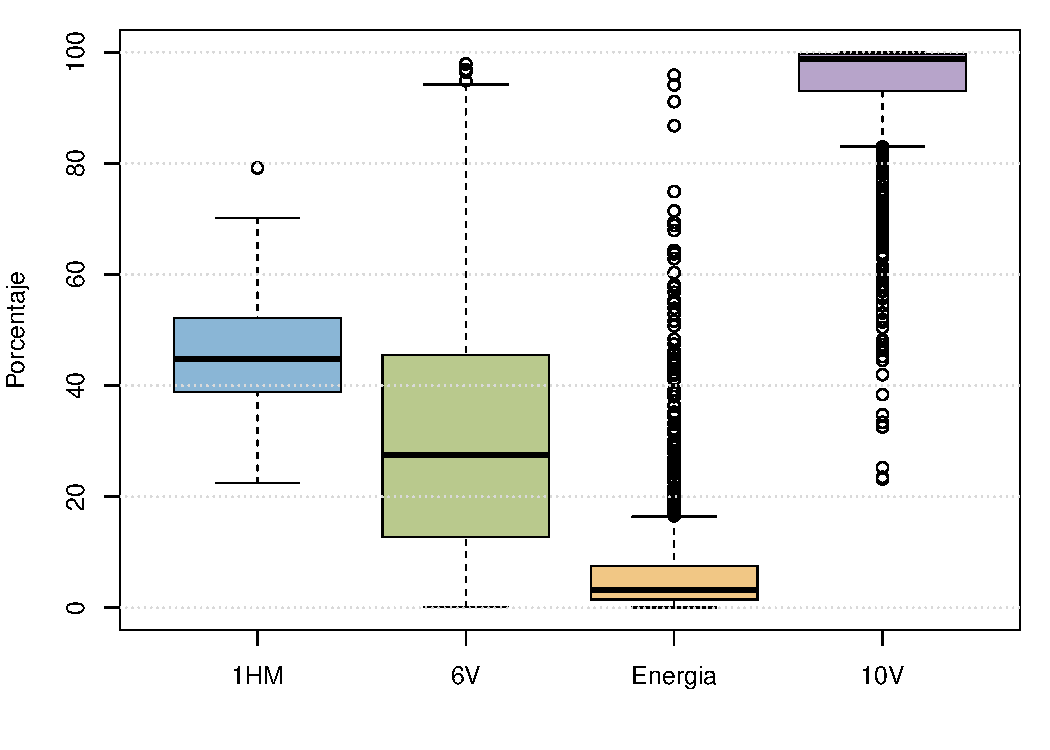
\includegraphics[width=.9\textwidth]{../../resultados/descriptivos_sensibilidades_20261018/figuras/distribuciones_cuatro.pdf}
\caption{Distribuciones de cuatro candidatas en el ámbito municipal e insular. Las cajas muestran mediana e intervalo intercuartílico; los bigotes se extienden hasta los datos dentro de 1,5 veces ese intervalo. Los puntos exteriores se conservan. Fuente: matriz recalculada de ocho indicadores.}
\end{figure}

\subsection{Sensibilidad de fórmulas y no respuesta}

La comparación utiliza las mismas unidades y define $\Delta_i=x_i^{(a)}-x_i^{(0)}$. Se reportan media de $|\Delta_i|$, máximo, número de casos con $|\Delta_i|\geq0,02$ y correlación entre rangos con empates promediados, $\rho_s=\operatorname{cor}(\operatorname{rango}(x^{(0)}),\operatorname{rango}(x^{(a)}))$. El umbral de dos puntos porcentuales es descriptivo, no un nivel de significancia. La exploración de supuestos de normalización y ponderación sigue las recomendaciones de transparencia y sensibilidad para indicadores compuestos \citep{oecd2008composite,decancq2013weights}.

En 5PM, con $U$ trabajo no remunerado, $B$ búsqueda, $C$ incapacidad y $V=T-NR$, la alternativa de peso $w\in\{1,2,3\}$ es
\begin{equation}
L_w=\frac{U+B+wC}{wV}=\frac{C}{V}+\frac{U+B}{wV}.
\end{equation}
La normalización por el peso máximo conserva el rango [0,1]: al aumentar $w$ mantiene el aporte normalizado de incapacidad y reduce el de las otras dos categorías. Por ello, los deltas reflejan conjuntamente ponderación relativa y normalización; no son cambios observados de actividad de la población.

Para gas e internet, si $N$ es carencia observada, $T$ total y $R$ no respuesta, se conservan:
\begin{equation}
p_{\text{válido}}=\frac{N}{T-R},\qquad
p_{\mathrm{inferior}}=\frac{N}{T},\qquad
p_{\mathrm{superior}}=\frac{N+R}{T}.
\end{equation}
Las cotas asignan a toda NR respectivamente ausencia o presencia de carencia. Son escenarios extremos de asignación, no intervalos de confianza. El denominador válido describe las respuestas observadas; extenderlo a todas las viviendas requeriría hipótesis sobre el mecanismo de NR que aquí no se asumen. Para 5PM, el escenario de cota asigna puntuación máxima a NR y normaliza por $2T$. Para 10V, incluir personas sin energía en el denominador cambia también la población objetivo: no es solo un ajuste de NR.

\begin{table}[htbp]
\centering\small
\caption{Sensibilidad de fórmulas en las 1.102 unidades municipales e insulares}\label{tab:sensibilidad_actual}
\begin{adjustbox}{max width=\textwidth}
\begin{tabular}{@{}lrrrr@{}}
\toprule
Alternativa & $\rho_s$ & $|\Delta|$ medio (pp) & $|\Delta|$ máx. (pp) & $\geq2$ pp \\
\midrule
5PM: peso 1:1 & 0,948 & 2,75 & 21,43 & 698 \\
5PM: peso 3:1 & 0,975 & 0,92 & 7,14 & 44 \\
5PM: total & 0,999 & 0,09 & 0,84 & 0 \\
5PM: cota NR & 0,858 & 1,79 & 18,26 & 216 \\
Gas: total & 0,994 & 0,54 & 12,46 & 52 \\
Internet: total & 0,968 & 0,75 & 14,01 & 69 \\
10V: total & 0,446 & 7,44 & 97,62 & 691 \\
17PM: Normal incompleta & 0,998 & 0,28 & 4,79 & 12 \\
17PM: base válida & 0,968 & 1,11 & 21,41 & 86 \\
\bottomrule
\end{tabular}

\end{adjustbox}
\par\footnotesize Fuente: \path{sensibilidades_formulas_por_ambito.csv}. Cada alternativa se compara con su fórmula principal. 17PM permanece fuera de las ocho candidatas; sus filas son exploratorias.
\end{table}

Al separar ANM cambia el conjunto de comparación respecto de la tabla histórica de 1.122 códigos: por ejemplo, los conteos del peso 5PM y del denominador 10V no deben trasladarse de una tabla a otra. El cambio a peso 1:1 tiene mayor efecto que el cambio a 3:1 bajo la normalización elegida; esa asimetría no demuestra que el peso dos sea óptimo. En 10V, la elevada sensibilidad revela que la interpretación condicionada al denominador es esencial. Las fórmulas aprobadas se conservan, con esas cautelas.

\begin{figure}[htbp]
\centering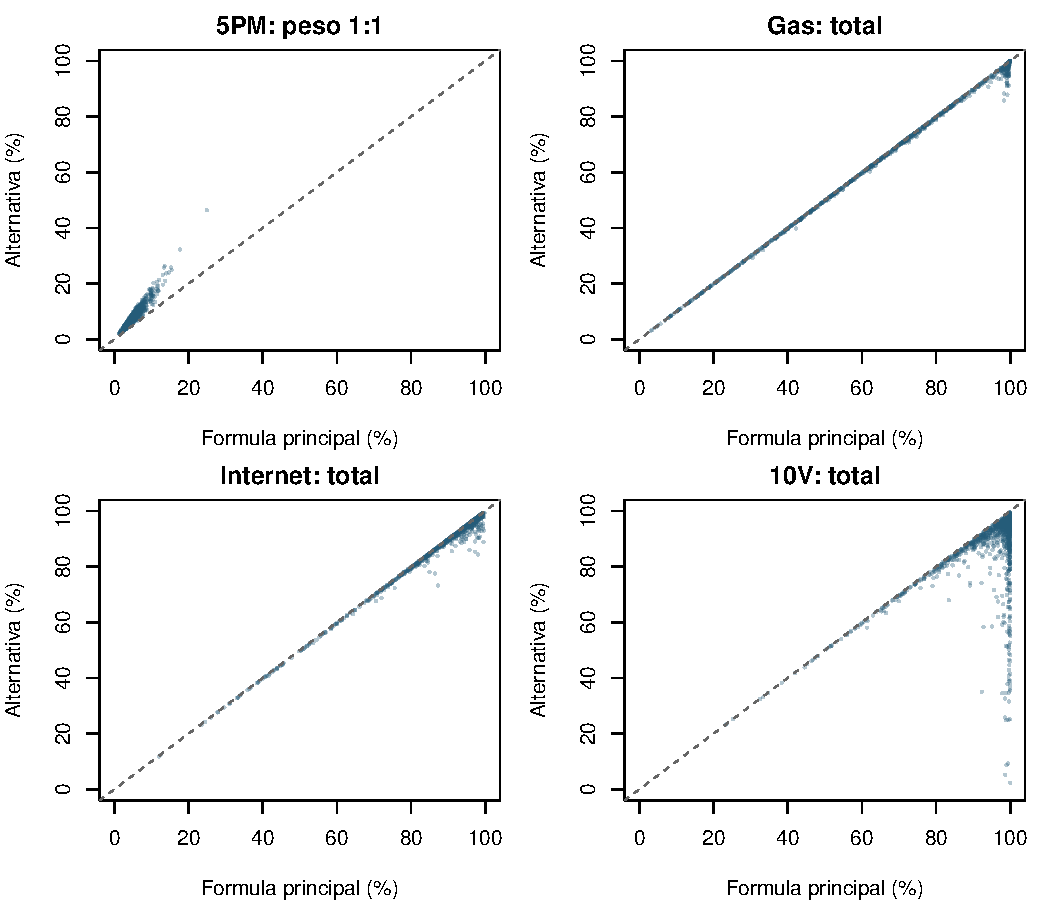
\includegraphics[width=.95\textwidth]{../../resultados/descriptivos_sensibilidades_20261018/figuras/sensibilidad_denominadores.pdf}
\caption{Fórmula principal frente a alternativas de peso y denominador. La diagonal indica igualdad; cada punto corresponde a una unidad municipal o insular. Fuente: sensibilidades por código.}
\end{figure}

\subsection{Sensibilidad de correlaciones, sin componentes principales}

Para evaluar efectos sobre las asociaciones se calculan matrices de Pearson y Spearman por escenario. Sobre los pares comunes $\mathcal{P}$ se resumen
\begin{equation}
\Delta_r^{\max}=\max_{(j,k)\in\mathcal P}|r_{jk}^{(a)}-r_{jk}^{(0)}|,\qquad
\mathrm{RDCM}_r=\sqrt{\frac{1}{|\mathcal P|}\sum_{(j,k)\in\mathcal P}(r_{jk}^{(a)}-r_{jk}^{(0)})^2}.
\end{equation}
Estas medidas describen cambios de asociación; no son contrastes de hipótesis. Spearman permite comprobar si las relaciones monotónicas difieren de las lineales; ninguna de las dos elimina por sí sola el efecto de agregación territorial ni garantiza una estructura dimensional adecuada \citep{jolliffe2002principal}.

En el escenario principal, Pearson entre 1HM y 2HM es $-0,721$, mientras que entre internet y 10V es $0,833$ (\path{correlaciones_escenarios.csv}). La primera relación indica estructuras territoriales de hogares contrapuestas, aunque ambas candidatas tengan dirección conceptual positiva; no implica corregir signos automáticamente. La segunda motiva evaluar redundancia estadística, aunque los conceptos difieran. Ninguna anticipa por sí sola cargas o dimensiones del PCA pendiente.

\begin{table}[htbp]
\centering\small
\caption{Cambios de correlación de Pearson bajo alternativas, sobre 28 pares comunes}\label{tab:corr_sensibilidad_actual}
\begin{adjustbox}{max width=\textwidth}
\begin{tabular}{@{}lrr@{}}
\toprule
Alternativa & Máximo $|\Delta r|$ & Raíz de diferencia cuadrática media \\
\midrule
5PM: peso 1:1 & 0,163 & 0,048 \\
5PM: peso 3:1 & 0,111 & 0,032 \\
5PM: total & 0,015 & 0,004 \\
5PM: cota NR & 0,335 & 0,090 \\
Gas: total & 0,015 & 0,004 \\
Internet: total & 0,047 & 0,013 \\
10V: total & 0,909 & 0,259 \\
Gas e internet: total & 0,047 & 0,013 \\
\bottomrule
\end{tabular}

\end{adjustbox}
\par\footnotesize Fuente: \path{sensibilidad_correlaciones.csv}. Las matrices completas y las versiones Spearman se conservan en \path{correlaciones_escenarios.csv}.
\end{table}

La alternativa de 10V modifica las asociaciones mucho más que las variantes de gas e internet. Eso motiva mantener visible la definición condicional y exigir sensibilidad dimensional en la siguiente fase. También se guardan matrices con basuras, 17PM, paredes desagregadas y retiro de candidatas próximas al IPM. Retirar o añadir columnas deja iguales las correlaciones entre las variables conservadas: un delta cero en esos pares es una identidad del cálculo, no evidencia de estabilidad de componentes o rankings. Evaluar esa estabilidad requiere el PCA, expresamente diferido.

\subsection{Valores extremos, integridad y cuestiones pendientes}

La matriz de ocho candidatas en el ámbito municipal e insular registra 43 códigos con 47 celdas cuyo $|z|>4$, usando la desviación convencional para mantener la regla histórica. El cotejo independiente con los valores cacheados del Excel identifica hoja, fila, numerador y denominador para cada celda: ninguna supera una diferencia de $10^{-12}$. Se preservan todas las observaciones. El detalle está en \path{cotejo_extremos_excel.csv}; confirmar la transcripción no valida el fenómeno en campo. Los 32 casos de la matriz histórica de siete variables pertenecen a otra especificación y no se sustituyen retrospectivamente por esta lista.

Los hash de los insumos antes y después coinciden, según \path{integridad_insumos.csv}; el cotejo del libro añade SHA-256 en \path{integridad_excel_cotejo.csv}. La salida \path{resumen_ejecucion.csv} registra ocho candidatas sin NA, cero diferencias de fórmula y PCA no ejecutado. La revisión bibliográfica corrigió el DOI de Kaiser y la autoría del artículo de Monsalvo Herrera y Jiménez a partir de las páginas editoriales. No se atribuye respaldo empírico al peso 2:1 ni a \enquote{No tiene estrato} que las fuentes no proporcionan.

Quedan pendientes la decisión final sobre San Andrés en el PCA municipal, los enlaces territoriales para SECOP, los diagnósticos de adecuación de la matriz definitiva, la retención e interpretación de componentes, la estabilidad de sus cargas y puntajes, y la regla de construcción del IVS. El trabajo actual cierra fórmulas, clasificación histórica ANM y evidencia descriptiva; el alcance de la justificación sigue siendo explícitamente parcial para las decisiones normativas. El CSV histórico conserva una instrucción residual en el campo de verificación de 6PM sobre desocupación: no se aplica, pues el acuerdo vigente excluye ese cuadro. La nota de actualización registra esa inconsistencia sin alterar el archivo histórico.


\section{Fórmulas de auditoría y pruebas estadísticas por etapa}
\label{sec:formulas_pruebas}
Esta sección presenta las expresiones aplicadas en el orden del flujo de trabajo. Se distingue entre procedimientos \textbf{ejecutados}, cuya evidencia está en scripts y salidas, y procedimientos \textbf{pendientes}, especificados para etapas futuras pero aún sin resultados para la matriz acordada. Los diagnósticos de una matriz anterior no se trasladan a la matriz candidata actual.

\subsection{Etapa 1. Verificación de estructura, llaves y cobertura}

Cada llave municipal se normaliza como texto de cinco dígitos, $c_i\in\{0,\ldots,9\}^5$. La consistencia departamental se evalúa con
\[
I_{D,i}=\mathbf{1}\{\texttt{codigo\_departamento}_i=\operatorname{substr}(c_i,1,2)\}.
\]
El control exige cero códigos duplicados y cero filas con $I_{D,i}=0$. La cobertura entre dos fuentes $A$ y $B$ se compara mediante la diferencia simétrica de conjuntos, $A\triangle B$. Para tablas con más de una fila municipal, la llave compuesta debe ser única: municipio--área--sexo, municipio--área--tipo de vivienda o municipio--área--grupo de edad, según el bloque.

La matriz de presencia define $P_{ij}=1$ cuando el código $i$ aparece en la fuente $j$, y $0$ en caso contrario. Las combinaciones de área, edad o tipo no publicadas por el diseño se cuentan como \emph{ausencias estructurales}, no como celdas faltantes ni como ceros imputados. El cruce histórico con DIVIPOLA actual identificaba 18 ANM. La verificación de la geografía de 2018 amplía la clasificación a veinte al incorporar Barrancominas y Mapiripana; se conservan separadas en la actualización descriptiva.

En reconciliaciones de conteos se calcula el residuo $e_i=T_i-\sum_{k=1}^{K}C_{ik}$, donde $T_i$ es el total publicado y $C_{ik}$ las categorías exhaustivas. Una fila viola la identidad si $|e_i|>0,5$ personas o viviendas. El rango de proporciones 0--1 se controla con $\mathbb{1}(x_i<0\ \text{o}\ x_i>1)$; para indicadores IPM se usa el rango [0,100]. La igualdad entre las columnas IPM Municipal e IPM se verifica con tolerancia $10^{-10}$. Los detalles por chequeo, hoja y tolerancia están en los CSV de verificación.

\subsection{Etapa 2. Construcción de indicadores candidatos}

Las expresiones usan conteos del CNPV 2018 del área \enquote{Total}. Para todo cociente se aplica $\operatorname{ratio}(a,b)=a/b$ si $b>0$; un denominador cero o indefinido genera NA y no un cero artificial.

\begin{singlespace}\small
\begin{longtable}{@{}p{0.15\textwidth}p{0.52\textwidth}p{0.23\textwidth}@{}}
\caption{Fórmulas operacionales de las candidatas}\label{tab:formulas_algebraicas}\\
\toprule
\textbf{Indicador} & \textbf{Fórmula operacional} & \textbf{Estado e interpretación}\\
\midrule
\endfirsthead
\toprule
\textbf{Indicador} & \textbf{Fórmula operacional} & \textbf{Estado e interpretación}\\
\midrule
\endhead
1HM & $H^{<15}_i/H_i$: hogares que reportan menores de 15 / hogares totales. & Candidato; proxy de carga potencial de cuidado, no dependencia económica.\\
2HM & $H^{60+}_i/H^{(2HM)}_i$: hogares con personas de 60+ / total de hogares del bloque 2HM. & Candidato; no mide dependencia funcional.\\
6V & $(G_i+T_i+M_i+C_i+D_i+S_i)/V_i$: Guadua, Tapia/bahareque/adobe, Madera burda, Caña/vegetales, Desecho y Sin paredes / viviendas tipo Total. & Candidato; agregado acordado, sin pesos por severidad.\\
8V energía & $E_i^{-}/E_i$: viviendas ocupadas presentes sin energía / total viviendas ocupadas presentes. & Candidato de carencia.\\
8V gas & $G_i^{-}/(G_i^{T}-G_i^{NR})$. & Candidato entre respuestas clasificables; NR se conserva y se sensibiliza.\\
8V internet & $I_i^{-}/(I_i^{T}-I_i^{NR})$. & Candidato entre respuestas clasificables; NR se conserva y se sensibiliza.\\
10V estrato & $(E_{1i}+E_{2i}+N_i)/(\sum_{s=1}^{6}E_{si}+N_i)$. & Candidato acordado; excluye Sin servicio y No sabe/No responde del cociente.\\
5PM actividad & $(U_i+B_i+2C_i)/[2(T_i-N_i)]$: negocio no remunerado, buscó trabajo, incapacidad permanente (peso 2), sobre respuestas válidas ponderadas. & Candidato experimental; no es tasa oficial ni dependencia del hogar.\\
17PM sin media completa & $(Ninguno+Preescolar+Primaria_{c/i}+Secundaria_{c/i}+Media_i)/P_{5+}$. & Descriptiva reservada; fuera del primer PCA.\\
\bottomrule
\end{longtable}
\end{singlespace}

En 5PM el denominador ponderado limita la puntuación a [0,1], bajo categorías exhaustivas y mutuamente excluyentes. El peso 2 para incapacidad es una decisión normativa del equipo, no una estimación del censo. En 17PM las proporciones de cada una de las 15 categorías son $p_{ik}=n_{ik}/P_{5+}$; se controla $|\sum_{k=1}^{15}p_{ik}-1|\leq10^{-10}$. La sensibilidad incorpora Normal incompleta al numerador; Normal completa se excluye. El denominador 5+ incluye Sin información en la fórmula principal, con alternativa que la excluye.

\subsection{Etapa 3. Controles aritméticos, rangos y completitud}

El residuo $e_i$ de la etapa 1 se aplica a los totales publicados y sus categorías: distribución educativa 17PM, actividad 5PM, nueve materiales 6V, energía 8V, gas e internet 8V y categorías 10V. Para la matriz candidata también se verifica cobertura/unicidad, que cada proporción esté en [0,1], y el número de valores NA. La ejecución del 15/10/2026 registró cero violaciones en los controles incluidos y 10.098 celdas completas para nueve candidatas en 1.122 unidades territoriales. Esto confirma coherencia aritmética y cobertura de la salida, no validez teórica del constructo.

En la auditoría del IPM, cada indicador se contrasta contra [0,100], se compara IPM Municipal con IPM, y se reconcilian las hojas ancha y largas por código y variable. Los resúmenes regionales, departamentales y controles se recalculan desde la tabla ancha y se informa su diferencia absoluta. El detalle por prueba está en \path{resultados/verificacion_consolidados/chequeos_consistencia.csv}; las discrepancias no se corrigen automáticamente.

\subsection{Etapa 4. Auditoría descriptiva, correlaciones y extremos}

Para cada variable $x$, se calculan media $\bar{x}=n^{-1}\sum_i x_i$, varianza muestral $s^2=(n-1)^{-1}\sum_i(x_i-\bar{x})^2$, mínimos, máximos y cuantiles tipo 7 de R (1\%, 25\%, 50\%, 75\%, 99\%). La función auxiliar define los momentos estandarizados como
\[
g_1=\frac{n^{-1}\sum_i(x_i-\bar{x})^3}{s^3},\qquad
g_2=\frac{n^{-1}\sum_i(x_i-\bar{x})^4}{s^4}-3,
\]
para asimetría y curtosis en exceso; el script de auditoría también genera esos dos descriptivos con \texttt{psych::describe}, cuya convención de corrección finita puede producir pequeñas diferencias. Se inspecciona porcentaje de ceros $100n^{-1}\sum_i\mathbf{1}(x_i=0)$ y varianza casi nula ($s^2<10^{-8}$). Los umbrales de alerta exploratoria son $|g_1|>2$, al menos 50\% de ceros, o proporciones fuera de [0,1]. No son pruebas de normalidad ni reglas automáticas de exclusión.

La matriz de correlaciones histórica es Pearson: $r_{jk}=\operatorname{cov}(X_j,X_k)/(s_js_k)$, calculada sobre la base total; en la auditoría se recalculó cada par y se comparó con el CSV, con tolerancia $10^{-10}$. Los niveles descriptivos fueron $|r|\geq0,40$ (moderado), $|r|\geq0,70$ (fuerte), y alertas $|r|\geq0,90$ y $|r|\geq0,95$. Estos umbrales no son contrastes de significancia.

La estandarización histórica se define como $z_{ij}=(x_{ij}-\bar{x}_j)/s_j$. Se marcó como extremo si $|z_{ij}|>4$ para al menos un indicador. La matriz previa de siete candidatos produjo 32 unidades con algún valor extremo. Es un indicador para cotejar la fuente, no una razón para corregir o eliminar observaciones. La actualización recalcula 43 códigos con 47 celdas extremas para ocho variables y 1.102 unidades municipales e insulares; el cotejo fuente se documenta en la sección de actualización descriptiva.

La auditoría reproducible de artefactos comprueba que los resultados almacenados coincidan con su recálculo. Para descriptivos se evalúa la máxima diferencia absoluta entre los valores guardados y recalculados de mínimo, percentil 1, mediana, media, percentil 99 y máximo; para correlaciones se usa la máxima diferencia por par. En ambos casos se exige diferencia menor que $10^{-10}$. Para sensibilidad NR se comparan los conteos de municipios marcados y la máxima diferencia absoluta entre resumen y archivo municipal; para extremos se compara el número de municipios con al menos un $|z|>4$. La auditoría histórica obtuvo diferencias de $1,11\times10^{-16}$ en descriptivos, $1,11\times10^{-16}$ en correlaciones y cero en los dos últimos controles: los cuatro controles aprobaron la conciliación de archivos. Esta verificación comprueba reproducción interna, no la validez del indicador.

\subsection{Etapa 5. Sensibilidad de fórmulas y no respuesta}

Para cada municipio se comparan la fórmula principal $a_i$ y la alternativa $b_i$. Se calcula diferencia absoluta $d_i=|a_i-b_i|$, correlación de rangos $\rho_s=\operatorname{cor}(rank(a),rank(b))$ en pares completos, diferencia máxima $\max_i d_i$, y número de unidades con $d_i\geq0,02$. En la auditoría histórica se definió además diferencia relativa $q_i=d_i/|a_i|$ cuando $a_i\ne0$; un municipio era sensible si $d_i\geq0,02$ \textbf{o} $q_i\geq0,10$. El resumen actual de escenarios que acompaña la matriz candidata usa el umbral absoluto de dos puntos porcentuales.

Los escenarios ejecutados son: 5PM con/sin No informa; cota que asigna puntuación máxima a No informa, $(U_i+B_i+2C_i+2N_i)/(2T_i)$; pesos de incapacidad 1:1 y 3:1; gas e internet con denominador válido frente al total publicado; 10V frente al total de personas de BU; y 17PM incluyendo Normal incompleta y excluyendo Sin información del denominador. En 5PM, la alternativa que mantiene numerador observado pero emplea total es $(U_i+B_i+2C_i)/(2T_i)$. En servicios, el escenario alterno divide el conteo sin servicio por el total que incluye Sin información. Los resultados numéricos están en la Tabla \ref{tab:sensibilidad}.

La tasa municipal de NR por ítem es $NR_i=n_{NR,i}/T_i$; la tasa agrupada ponderada es $\sum_i n_{NR,i}/\sum_i T_i$. Se reportan máximo municipal y unidades que exceden los umbrales 5\%, 10\% y 20\%. \enquote{No tiene estrato} es sustantiva, no NR; \enquote{No sabe/No responde} se conserva como categoría no clasificable. Las comparaciones de valores y rangos por municipio no establecen la estabilidad de correlaciones, KMO/MSA, cargas o puntajes.

\subsection{Etapa 6. Adecuación para PCA: fórmulas, resultados y pendientes}

El índice KMO global contrasta la suma de correlaciones ordinarias $r_{ij}$ con las correlaciones parciales $a_{ij}$:
\[
KMO=\frac{\sum_{i<j}r_{ij}^{2}}{\sum_{i<j}r_{ij}^{2}+\sum_{i<j}a_{ij}^{2}}.
\]
El MSA individual para la variable $i$ es $MSA_i=\sum_{j\ne i}r_{ij}^{2}/[\sum_{j\ne i}r_{ij}^{2}+\sum_{j\ne i}a_{ij}^{2}]$. Las correlaciones parciales controlan linealmente las restantes variables. KMO/MSA describen la proporción de correlación simple frente a parcial; son diagnósticos y no una aprobación automática \citep{kaiser1974simplicity}.

La prueba de esfericidad de Bartlett contrasta $H_0:R=I_p$ frente a correlaciones no identidad. El estadístico usado por la implementación es
\[
\chi^2_B=-\left[n-1-\frac{2p+5}{6}\right]\ln|R|,\qquad gl=\frac{p(p-1)}{2},
\]
donde $n$ es el número de unidades, $p$ el número de indicadores y $|R|$ el determinante de la matriz de correlaciones. Un p-valor pequeño evidencia que $R$ difiere de identidad; no demuestra que exista un IVS unidimensional interpretable. Con $n$ grande puede resultar significativo ante asociaciones pequeñas \citep{bartlett1950factor}.

La aproximación inferencial de Bartlett presupone condiciones de muestreo e independencia y un modelo de normalidad multivariada. En agregados censales territoriales, con proporciones acotadas y posible dependencia espacial, no debe interpretarse como una prueba de representatividad ni como aprobación automática del índice. La transformación PCA exploratoria puede calcularse sin exigir normalidad; las garantías inferenciales de un contraste son una cuestión distinta \citep{jolliffe2002principal}.

\begin{table}[htbp]
\centering\small
\caption{Estado de las pruebas de adecuación multivariada}\label{tab:estado_pruebas_pca}
\begin{adjustbox}{max width=\textwidth}
\begin{tabular}{@{}p{0.20\textwidth}p{0.25\textwidth}p{0.40\textwidth}p{0.10\textwidth}@{}}
\toprule
\textbf{Prueba} & \textbf{Matriz} & \textbf{Resultado documentado} & \textbf{Estado}\\
\midrule
KMO global & Histórica, 7 variables & 0,642484; adecuación moderada, no aprobación automática. & Ejecutado\\
Bartlett & Histórica; $n=1122$, $p=7$ & $\chi^2=4664,8728$, $gl=21$; archivo almacena $p=0$ por subdesbordamiento, se informa $p<0,001$. & Ejecutado\\
MSA por variable & Histórica, 7 variables & Estrato 1--2: 0,414311, el MSA más bajo; otros valores en \path{resultados/base_trabajo/kmo_por_indicador.csv}. & Ejecutado\\
KMO/Bartlett & Ocho candidatas; $n=1102$ & KMO 0,672406; $\chi^2=4305{,}6886$, $gl=28$, $p$ nominal $<0,001$; MSA 0,5553--0,7842. & Ejecutado 20/10\\
Sensibilidad de adecuación & Fórmulas y ámbitos alternativos & KMO/MSA ejecutados 20/10; cargas, componentes y puntajes aún diferidos. & Parcial\\
Estabilidad PCA & Fórmulas y universos alternativos & Componentes, cargas, eigenvalores y puntuaciones aún no calculados. & Pendiente\\
\bottomrule
\end{tabular}
\end{adjustbox}
\end{table}

Los resultados KMO/Bartlett disponibles pertenecen a una versión previa de siete candidatos: actividad, energía, gas, recolección de basuras, internet, hogares con menores y estrato 1--2. No corresponden a las nueve candidatas calculadas más recientemente ni a las ocho variables acordadas para el primer PCA. Los 21 grados de libertad son coherentes con $p=7$. El p-valor registrado como cero es una limitación de representación numérica, no probabilidad exactamente nula. El diagnóstico del 20 de octubre ya recalcula estas pruebas para las ocho candidatas y el ámbito municipal e insular; si cambia la especificación final, deben repetirse.

\subsection{Trazabilidad y límites}

Las expresiones y controles anteriores se vinculan con \path{R/02_base_final_indicadores.R}, \path{R/03_auditoria_indicadores.R}, \path{R/05_conformar_indicadores_finales.R}, la configuración \path{R/00_config.R} y sus CSV. Los indicadores y sensibilidades históricos se reproducen desde \path{resultados/indicadores_finales_ivs_20261015/}. Los valores históricos de KMO, Bartlett y MSA pertenecen a la matriz de siete variables; los nuevos resultados de ocho candidatas se documentan por separado en la actualización del 20 de octubre. La actualización descriptiva añade fórmulas, correlaciones y extremos mediante el script 06; no ejecuta PCA. Los chequeos estructurales de los consolidados están desglosados por hoja en \path{resultados/verificacion_consolidados/}. No se ha ejecutado PCA ni se ha validado un IVS final.



\section{Preparación para el PCA y estado del IVS}
\label{sec:pca_estado}
\subsection{Matrices disponibles y especificación del primer PCA}

La corrida del 15 de octubre creó \path{matriz_pca_candidata.csv} en escala 0--1 y \path{matriz_pca_candidata_z.csv} con nueve variables estandarizadas. Estas son matrices de preparación, no resultados de componentes ni un índice. La decisión posterior de reservar 17PM implica que el primer PCA use las ocho candidatas restantes. Se debe filtrar esa columna y volver a estandarizar las ocho variables en el universo municipal definido; no se debe utilizar sin cambios el archivo z de nueve variables ni suponer que su PCA equivale al modelo acordado.

La matriz histórica cubre 1.122 códigos territoriales. La actualización del 18 de octubre crea una base descriptiva de ocho variables para 1.101 municipios/distritos y San Andrés, con veinte ANM identificadas aparte. Se conservan todos los códigos en otra salida. Antes del PCA debe cerrarse la participación de la unidad insular y estandarizarse nuevamente el universo elegido. La actualización actual no produce componentes, cargas ni puntajes.

\subsection{Secuencia recomendada de diagnóstico}

El análisis exploratorio se realizará sobre la matriz z de ocho variables y el universo depurado, siguiendo una secuencia reproducible:
\begin{enumerate}[leftmargin=1.27cm]
  \item confirmar completitud, variabilidad no nula, rangos y dirección;
  \item examinar distribuciones, correlaciones y observaciones influyentes, cotejando extremos con fuente sin eliminarlos automáticamente;
  \item estudiar adecuación con matriz de correlación, KMO/MSA y Bartlett como diagnósticos complementarios, no como umbrales que por sí solos aprueban PCA;
  \item ejecutar PCA y conservar valores propios, varianza explicada, cargas y puntajes con código, semilla si corresponde, y versión de la matriz;
  \item seleccionar componentes con evidencia conjunta: gráfico de sedimentación, análisis paralelo, interpretabilidad y estabilidad; no depender exclusivamente de la regla de eigenvalor mayor que uno \citep{horn1965rationale,jolliffe2002principal};
  \item comparar resultados bajo sensibilidades de no respuesta, peso 5PM, inclusión de 17PM y universo territorial;
  \item solo si la solución resulta interpretable y estable, evaluar si procede un índice unidimensional o una puntuación multidimensional.
\end{enumerate}

KMO resume la proporción de correlación parcial y Bartlett contrasta la hipótesis de matriz identidad; en un universo grande, la significancia de Bartlett puede aparecer ante asociaciones pequeñas. Por eso se interpretarán junto con magnitud de correlaciones, MSA por variable, estabilidad y sentido sustantivo. El número de componentes se decidirá mediante evidencia comparada y no se fijará de antemano.

\subsection{IPM como contraste externo}

El IPM municipal no participa en el cálculo de los componentes. Después de definir una solución, podrá examinarse concordancia de puntajes o rankings con el IPM, describiendo explícitamente los solapamientos conceptuales restantes. Esta asociación sería evidencia convergente parcial, no una validación definitiva ni un criterio para cambiar cargas automáticamente. Estudios territoriales que analizan IPM y estructura espacial sirven de antecedente aplicado, pero no demuestran por sí solos que la estructura del IVS propuesto sea válida \citep{monsalvo2025ipm}.

\subsection{Estado explícito}

\begin{center}
\begin{tabular}{@{}ll@{}}
\toprule
\textbf{Producto} & \textbf{Estado al 18/10/2026}\\
\midrule
Indicadores candidatos 0--1 & Ocho recalculados; educación reservada aparte \\
Matriz estandarizada z & Histórica de nueve columnas; nueva definitiva pendiente \\
Descriptivos y sensibilidad & Actualizados; incluye cambios en correlaciones \\
Primer PCA con ocho candidatas & Diferido por instrucción del equipo \\
Componentes, cargas y scores & Sin ejecución en esta entrega \\
IVS final y validado & No construido \\
Contraste externo IPM & Pendiente \\
Integración SECOP II 2026 & Pendiente; sin base integrada en este flujo \\
\bottomrule
\end{tabular}
\end{center}


\section{Limitaciones, decisiones abiertas y plan de trabajo}
\label{sec:limitaciones_pendientes}
\subsection{Limitaciones interpretativas}

\begin{itemize}[leftmargin=1.27cm]
  \item El CNPV mide condiciones de 2018; no representa por sí solo el contexto socioeconómico de 2026.
  \item La unidad territorial y el cambio de límites entre 2018 y 2026 generan una incompatibilidad potencial. Los códigos 27493 y 94663 requieren crosswalk verificable antes de comparar contratación.
  \item Las veinte ANM de 2018 se identifican y se describen aparte. El ámbito descriptivo principal incluye municipios/distritos y San Andrés; su inclusión insular en el futuro PCA requiere decisión explícita.
  \item Hogares con menores y con personas mayores son proxies de carga potencial de cuidado, no mediciones de dependencia funcional, económica o de necesidad de cuidado.
  \item 5PM agrupa situaciones heterogéneas y usa una ponderación normativa 2:1. El indicador no es una tasa oficial de desempleo ni describe actividad de un hogar.
  \item El estrato es una clasificación del inmueble para servicios, no una medida directa de ingreso. La inclusión de \enquote{No tiene estrato} como condición de vulnerabilidad es una decisión del equipo, cuya sensibilidad al denominador es alta.
  \item 17PM usa población 5+ y no controla composición de edad. Se excluye del primer PCA y se reserva para sensibilidad exploratoria.
  \item La matriz z equaliza varianzas, pero no corrige asimetría, observaciones influyentes, error conceptual o solapamiento entre indicadores.
  \item No se han actualizado KMO, Bartlett, MSA, análisis paralelo ni estabilidad para las ocho candidatas y el universo municipal final.
  \item SECOP II no se ha integrado. La comparación 2018--2026 será temporalmente asimétrica y ecológica; los resultados describirán asociación, no causalidad.
\end{itemize}

\subsection{Decisiones adoptadas y asuntos abiertos}

\begin{table}[htbp]
\centering\small
\caption{Estado de decisiones metodológicas}\label{tab:decisiones_pendientes}
\begin{adjustbox}{max width=\textwidth}
\begin{tabular}{@{}p{0.32\textwidth}p{0.28\textwidth}p{0.32\textwidth}@{}}
\toprule
\textbf{Decisión / asunto} & \textbf{Estado} & \textbf{Siguiente acción}\\
\midrule
IVS con indicadores DANE; SECOP como análisis posterior & Acordado & Mantener separados los bloques de vulnerabilidad y contratación. \\
Base censal 2018; SECOP II prioriza 2026 & Acordado & Documentar desfase temporal y cobertura. \\
ANM por fuera del IVS municipal principal & Lista histórica verificada; base separada & Cerrar tratamiento de San Andrés para el PCA. \\
27493 hacia 27615 para armonización & Decisión de enlace del equipo & Verificar límites/fuente oficial; no alterar 2018. \\
94663 hacia 94343 para armonización & Decisión de enlace del equipo & Agregar componentes de 2018 a geografía común antes de tasas, si el diseño de enlace lo requiere. \\
Cobertura SECOP 100\% del universo acordado & Criterio del equipo & Fijar denominador después de resolver universo y crosswalk. \\
5PM peso 2 para incapacidad & Aprobado como ponderación experimental & Reportar sensibilidad 1:1 y 3:1; no presentarlo como peso empírico. \\
17PM fuera del primer PCA & Acordado & Comparar luego solución de ocho variables con variante educativa, si se valida su universo. \\
Basuras fuera de las ocho & Confirmado el 18 de octubre & Conservar únicamente como sensibilidad exploratoria. \\
Solapamiento con IPM & Criterio acordado; matriz conceptual documentada & Contrastar después soluciones con retiro de candidatas cercanas. \\
PCA / IVS / validación externa / SECOP & Pendientes & Ejecutar en etapas, con diagnósticos y trazabilidad versionados. \\
\bottomrule
\end{tabular}
\end{adjustbox}
\end{table}

\subsection{Próximas etapas}

\begin{enumerate}[leftmargin=1.27cm]
  \item Cerrar la inclusión insular en el universo del PCA y verificar el crosswalk 2018--2026; la clasificación de veinte ANM ya está documentada.
  \item Seleccionar el ámbito definitivo desde las matrices de ocho variables y volver a estandarizarlo; preservar el escenario separado para ANM.
  \item Calcular KMO/MSA y Bartlett cuando se autorice la etapa multivariada. Los controles de fórmula, descriptivos, correlaciones y cotejo de extremos del ámbito municipal e insular ya se documentan en esta actualización.
  \item Ejecutar PCA exploratorio, comparar criterios de retención e inspeccionar estabilidad de cargas y puntajes bajo sensibilidades previamente definidas.
  \item Si la solución es interpretable y estable, formalizar la regla de construcción del IVS; posteriormente contrastarlo con IPM como criterio externo.
  \item Obtener SECOP II 2026, documentar cobertura municipal y armonizar límites antes de analizar asociación, correspondencia y brechas.
\end{enumerate}

La secuencia es consistente con guías de construcción de indicadores compuestos: las decisiones de normalización, ponderación, agregación y análisis de incertidumbre deben ser transparentes y evaluarse antes de interpretar un ranking \citep{oecd2008composite}. El IVS no se considerará terminado solo por obtener una primera componente principal.

